\documentclass{whutmod}
\usepackage[linesnumbered,ruled,lined]{algorithm2e}
\bibliographystyle{unsrt}
\team{A010}
\membera{刘子川}
\joba{编程}
\memberb{程宇}
\jobb{建模}
\memberc{祁成}
\jobc{写作}
\hypersetup{
	colorlinks=true,
	linkcolor=black
}


\newcommand{\upcite}[1]{\textsuperscript{\cite{#1}}}
%%%%%%%%%%%%%%%%%%%%%%%%%%%%%%%%%题目%%%%%%%%%%%%%%%%%%%%%%%%%%%%%%%%%%%%
\title{基于xxxxxxxx模型}
\tihao{1} 

\begin{document}

	\maketitle
	\thispagestyle{empty}
%%%%%%%%%%%%%%%%%%%%%%%%%%%%%%%%%摘要%%%%%%%%%%%%%%%%%%%%%%%%%%%%%%%%%%%%
	\begin{abstract}
		控制高压油管的压力变化对减小燃油量偏差,提高发动机工作效率具有重要意义。本文建立了基于质量守恒定理的微分方程稳压模型,采用二分法、试探法以及自适应权重的蝙蝠算法对模型进行求解。
		//
	
		针对问题一,建立基于质量守恒定律的燃油流动模型,考察单向阀开启时间对压力稳定性的影响。综合考虑压力与弹性模量、密度之间的关系,提出燃油压力-密度微分方程模型和燃油流动方程。本文采用改进的欧拉方法对燃油压力-密度微分方程求得数值解;利用二分法求解压力分布。综合考虑平均绝对偏差等反映压力稳定程度的统计量,求得直接稳定于100MPa的开启时长为\textbf{0.2955ms} ,在2s、5s内到达并稳定于150MPa时开启时长为\textbf{0.7795ms}、\textbf{0.6734ms},10s到达并稳定于150MPa的开启时长存在多解。最后对求解结果进行灵敏度分析、误差分析。
		//
	
		针对问题二,建立基于质量守恒定律的泵-管-嘴系统动态稳压模型,将燃油进入和喷出的过程动态化处理。考虑柱塞和针阀升程的动态变动,建立喷油嘴流量方程和质量守恒方程。为提高角速度求解精度,以凸轮转动角度为固定步长,转动时间变动步长,采用试探法粗略搜索与二分法精细搜索的方法求解,求得凸轮最优转动角速度\textbf{0.0283rad/ms(转速270.382转/分钟)},并得到该角速度下高压油管的密度、压力周期性变化图。对求解结果进行误差分析与灵敏度分析,考察柱塞腔残余容积变动对高压油管压力稳态的影响。
		//
	
		针对问题三,对于增加一个喷油嘴的情况,改变质量守恒方程并沿用问题二的模型调整供、喷油策略,得到最优凸轮转动角速度为\textbf{0.0522rad/ms(498.726转/分钟)};对于既增加喷油嘴又增加减压阀的情况,建立基于自适应权重的蝙蝠算法的多变量优化模型,以凸轮转动角速度、减压阀开启时长和关闭时长为参数,平均绝对偏差MAD为目标,在泵-管-嘴系统动态稳压模型的基础上进行求解,得到最优参数:\textbf{角速度0.0648 rad/ms(619.109转/分钟)}、减压阀的开启时长\textbf{2.4ms}和减压阀的关闭时长\textbf{97.6ms}。
		//
	
		本文的优点为:1. 采用试探法粗略搜索与二分法精细搜索结合的方法,降低了问题的求解难度。2.以凸轮转动角度为固定步长,对不同角速度按照不同精度的时间步长求解,大大提高了求解的精确度。 3.针对智能算法求解精度方面,采用改进的蝙蝠算法,使速度权重系数自适应调整,兼顾局部搜索与全局搜索能力。
		
		\keywords{
			微分方程\quad
			微分方程\quad	
			微分方程\quad
			微分方程\quad
		}
	\end{abstract}


%%%%%%%%%%%%%%%%%%%%%%%%%%%%%%%%%目录%%%%%%%%%%%%%%%%%%%%%%%%%%%%%%%%%%%%
	\thispagestyle{empty}
	\tableofcontents
	\setcounter{page}{0}                                               
	\newpage	%换页符
	

	
	\section{问题重述}	
		\subsection{问题背景}
	    	分析研究\upcite{1}。xxxxxxxxxxx\footnote{\quad xxxxxxxxxx.}.
	村通自来水工程是指在现有农村居民饮水安全工程的基础上,通过扩网、改造、联通、整合和新建等措施,把符合国家水质标准的自来水引接到行政村和有条件的自然 村,形成具有高保证率和统一供水标准的农村供水网络,基本形成覆盖全县农村的供水安全保障体系,实现农村供水由点到面、由小型分散供水到适度集中供水、由 解决水量及常规水质到水量、水质、水压达标等方面的提升,使广大农村居民长期受益,实现我县农村饮水“提质增效升级”的目的。
	
	自来水管道铺设是搭建自来水系统的重要环节,合理的管道铺设方案可以大幅度节约成本。本问题要求在充分考虑市场因素后,研究用两种不同型号的管道铺设该村的自来水管道的方案,使得建设成本降低。由于不同类形的管道的成本不同,且在实际应用中自来水厂有功率限制,研究自来水管的铺设对于村通自来水工程有着重要意义。
	
		\subsection{问题概述}
		    围绕相关附件和条件要求,研究两种型号的管道在各自来水厂间的铺设方案,依次提出以下问题:
		    
			\textbf{问题一:}
			设计从中心供水站A出发使得自来水管道的总里程最少的铺设方案,并求出该方案下I型管道和II型管道总里程数。
			
			\textbf{问题二:}
			由于二型管道数量不足,设计自来水厂升级方案使得两个二级自来水厂升级为一级自来水厂,使得二级管道的使用量尽可能减小。
			
			\textbf{问题三:}
            考虑自来水厂的功率限制,设计升级方案使得若干的二级自来水厂升级为一级,并求解该情况下的最小铺设总长度。
	
	\section{模型假设}
		\begin{itemize}                                             
		\item [(1)] 
		\item [(2)]
		\item [(3)] 
		\item [(4)] 
		\end{itemize}

		
	\section{符号说明}
		\begin{table}[H]
		\centering
		\setlength{\tabcolsep}{12mm}
		\begin{tabular}{cc}
			\toprule[1.5pt]
			\multicolumn{1}{m{5cm}}{\centering 符号} & \multicolumn{1}{m{5cm}}{\centering 说明} \\
			\midrule[1pt]		
			$P_n$  & 20个站点  \\ 
			$P_n$  & 20个站点  \\ 
		   	$P_n$  & 20个站点  \\ 
			\bottomrule[1.5pt]
		\end{tabular}
		\begin{tablenotes}
		\item 注:表中未说明的符号以首次出现处为准
		\end{tablenotes}
		\end{table}

	\section{问题一模型的建立与求解}
		\subsection{问题描述与分析}
			问题一要求分析一级供水站与二级供水站的分布情况,并根据分析结果,设计从中心供水站出发总里程最少的管道铺设方案。该问题本质是一个带特殊约束的最小生成树问题,即在不考虑二级供水站的情况下,一级供水站要相互连通。针对该问题,本组将供水站间的距离关系转化为权重矩阵,并设计二阶Prim算法以求解管道使用总里程最小的铺设方案。
			
		
			\begin{figure}[H]
				\centering
				
\includegraphics[width=\textwidth]{figures/whut.jpg}
				\caption{问题一思维流程图}\label{lct}
			\end{figure}
			
		\subsection{模型的建立}
		在村村通自来水工程的连通图$G=(V(G),E(G))$中,每个供水站可以视作一个节点$v \in V$,即对于中心供水站$v_0 \in V_0$、一级供水站$v_1(i) \in V_1 (i=1,2,\cdots,12)$ 和二级供水站$v_2(i) \in V_2 (i=1,2,\cdots,168)$,有$V(G)=V_0\cup  V_1\cup V_2$。节点间的供水管道看作边$e \in E(G)$。由中心供水站于一级供水站间可构成生成树:
		\begin{gather*}
		T_{1}=(V(T_{1}),E(T_{1})),
		\end{gather*}
		其中$T_{1}$代表一级生成树,其中$V(T_{1})=V_0\cup  V_1$,即一级生成树中的节点只包含中心供水站和一级供水站。
		
		在一级生成树生成树$T_1$的基础上引入二级站点$V_2$构成二级生成树:
		\begin{gather*}	
		T_{2}=(V(T_{2}),E(T_{2})),
		\end{gather*}
		其中$V(T_{2})=V(T_{1})\cup V_2$,且满足$E(T_{1})\subseteq  E(T_{2})$,且在任意生成树$T$中,都有$|E(T)|=|V(T)|-1$,即边数量为节点数量减一。
		
		边$e$的代价是两节点$v_a(i_1), v_b(i_2)$间的欧式距离,可表示为:
		\begin{gather}
		cost_{k}(v_a(i_1),v_b(i_2))=\left | v_a(i_1)-v_b(i_2) \right |,
		\end{gather}
		其中$a,b=0,1,2$,分别表示中心与一、二级供水站。$k=1,2$分别表示I型与II型管道,即有
			\begin{gather}
			k=\left\{\begin{matrix}1,a+b\leqslant 2
			\\ 2,a+b>2
			\end{matrix}\right.
			\end{gather}
		
		%由于I级和II级供水站的本质区别是II级供水站不能与中心供水站直接相连,故本问题实质上是一个二阶最小生成树问题。
		
		
		%我们以两节点间的欧式距离作为边的代价,应用改进的Prim算法(二阶的,想个名字!!!!!!)求解模型。
		%其思维流程图如图~\ref{lct}~所示:
		
			%同一般的最小生成树问题不同,问题一中的II级供水站生成树优化需待I级供水站的最小连通树生成后才能开始进行。因此,问题一的模型(取个屌点的名字?????)分为两部分,I级供水站和II级供水站先后进行目标优化。
			%本问题中,
			在此二阶最小生成树问题中,已知节点和边的关系为$|E(T)|=|V(T)|-1, $。即决策变量可表示为生成树的边集合:
			%生成树节点对应的序列作为决策变量,以序列矩阵的形式表示,每一层的最优序列矩阵可以表示为
			\begin{gather}
			E(T_k)=
			\begin{bmatrix}
			(v_{11} ,v_{12}) \\ 
			(v_{21} ,v_{22} )\\ 
			...,...\\
			(v_{|E(T_k)|,1},v_{|E(T_k)|,2})\\
			\end{bmatrix},k=1,2
			\end{gather}
			其中,$v_{i1}, v_{i2}(i =1,2,\cdots,|E(T_k)|)$分别代表边$e_i$的端点,且满足$E(T_1)\subseteq E(T_2)$,即生成树$T_1$优先生成并满足:
			\begin{gather}
			\sum_{i\in E(T_1) }cost_1(v_{i1},v_{i2})=\min\left \{ 	\sum_{i\in E(T_1) }cost_1(v_{i1},v_{i2}) \right \}
			\end{gather}
			即必须确保I型管道铺设距离最短,即保证一级生成树$T_1$为中心供水站和一级供水站构成的最小生成树。
			 %分别将I、II管道总里程作为优化目标,可知总里程是所有边的代价之和,而代价可以表示成节点间的距离,最佳节点序列已经存放在最优序列矩阵中,这些节点距离可以通过节点序列取出。
			 同时,总里程是关于$E_{i}$的函数。在二级生成树中对I型与II型管道的铺设距离求总和,可得目标函数即最短铺设总距离为:
			\begin{gather}
	         	\sum_{i\in E(T_2) }cost_1(v_{i1},v_{i2})+\sum_{i\in E(T_2) }cost_2(v_{i1},v_{i2})
			\end{gather}
			
			此问题的约束条件为问题一中的二级供水站生成树优化不能先于一级供水站的最小连通树生成,即对应总模型的数学描述为:
			\begin{gather}
			\min \left\{ \sum_{i\in E(T_2) }cost_1(v_{i1},v_{i2})+\sum_{i\in E(T_2) }cost_2(v_{i1},v_{i2}) \right \}
			\end{gather}
			\begin{gather*}
			s.t.\left\{\begin{matrix}
			E(T_{1})\subseteq  E(T_{2})\\ 
				\sum_{i\in E(T_1) }cost_1(v_{i1},v_{i2})=\min\left \{ 	\sum_{i\in E(T_1) }cost_1(v_{i1},v_{i2}) \right \} 
						\end{matrix}\right.
			\end{gather*}
		\subsection{模型的求解}
		为求取管道最小里程和最优路径,我们需要求解每一层的最优序列矩阵。针对问题一,我们采用Prim算法,分别实现由中心供水站到I级供水站、由I级供水站到II级供水站的最小生成树,可以求得每一层的最优序列矩阵$E(T_k)$。
		
		Prim算法的流程流程图如图~\ref{dsf}~所示
		\begin{figure}[H]
		\centering
		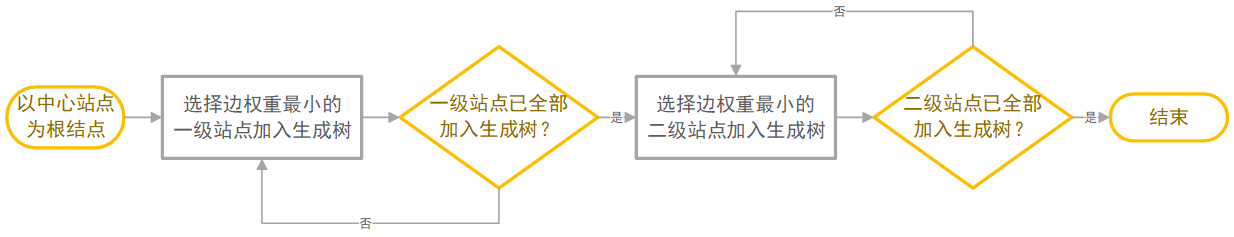
\includegraphics[width=\textwidth]{figures/a1.png}
		\caption{问题二思维流程图}\label{dsf}
	\end{figure}
		
        \subsection{实验结果及分析}
  1.灵敏度分析;(2.对比分析);3.算法收敛性分析;4.算法时间复杂度分析。。。
	\section{问题二模型的建立与求解}
		\subsection{问题描述与分析}	
			问题二要求升级两个II级供水站为I级供水站,使得II级管道里程数最少。
			
			\subsection{模型的建立}
			其中,第一层更新后的决策变量仍是最优节点序列,用最优序列矩阵表示为:
			\begin{gather}
			E(T_1')=
			\begin{bmatrix}
			(v_{\left | E(T_{1}')\right |,1},v_{\left | E(T_{1}')\right |,2})
			\end{bmatrix}
			\end{gather}
			其中,$v_{\left | E(T_{1}')\right |,1},v_{\left | E(T_{1}')\right |,2}$是由II级供水站升级成的I级供水站。此时约束条件仍是生成树$T_1$优先生成并满足
			\begin{gather}
			\sum_{i\in E(T_1) }cost_1(v_{i1},v_{i2})=\min\left \{ 	\sum_{i\in E(T_1) }cost_1(v_{i1},v_{i2}) \right \}
			\end{gather}
			目标函数为II级管道的总里程
			\begin{gather}
			\sum_{i\in E(T_2) }cost_2(v_{i1},v_{i2})=\min\left \{\sum_{i\in E(T_2) }cost_2(v_{i1},v_{i2})\right\}
			\end{gather}
			结合上述决策变量、目标函数、约束条件,得到以两个升级后的I级供水站为决策变量,以II级管道的总里程为目标函数,生成树$T_1$优先生成为约束条件的优化模型:
			\begin{gather}
			\min \left\{ \sum_{i\in E(T_2) }cost_2(v_{i1},v_{i2}) \right \}
			\end{gather}
			\begin{gather*}
			s.t.\left\{\begin{matrix}
			E(T_{1})\subseteq  E(T_{2})\\ 
			\sum_{i\in E(T_1) }cost_1(v_{i1},v_{i2})=\min\left \{ 	\sum_{i\in E(T_1) }cost_1(v_{i1},v_{i2}) \right \} 
			\end{matrix}\right.
			\end{gather*}
    		其思维流程图如图~\ref{lssssct}~所示:

			\begin{figure}[H]
				\centering
				
\includegraphics[width=\textwidth]{figures/whut.jpg}
				\caption{问题二思维流程图}\label{lssssct}
			\end{figure}


		
		\subsection{模型的求解}

        \subsection{实验结果及分析}
        
			结果如下表\ref{zhuanssssasgzai}所示:
			\begin{table}[H]
			\setstretch{1.4}  %设置表的行间距
			\centering		
			\caption{xxxxxxxxxxxxxxxxxxxxx}\label{biao1}
			\begin{tabular}{cc}
			\toprule[2pt]
				\multicolumn{1}{m{5cm}}{\centering xxxxxxx}
				& \multicolumn{1}{m{5cm}}{\centering xxxxxxx}
				\\
				\midrule[1pt]
				xxxxxxx &   909.80\\ 
				xxxxxxx & 	852.60\\ 
			\bottomrule[2pt]	
			\end{tabular}
			\end{table}
  
  			由表\ref{biao1}可知

			其各个小车的运输细节图下图所示:
			\begin{figure}[H]
				\centering
				\subfigure{
\includegraphics[height=8cm,width=7.5cm]{figures/whut.jpg}}
				\subfigure{
\includegraphics[height=8cm,width=7.5cm]{figures/whut.jpg}}
			\end{figure}	
			\begin{figure}[H]	
				\centering
				\subfigure{
\includegraphics[height=8cm,width=7.5cm]{figures/whut.jpg}}
				\subfigure{
\includegraphics[height=8cm,width=7.5cm]{figures/whut.jpg}}
				\caption{xxxxxxxxxxxxxxxxxxxxxxxxx}
				\label{fisg}
			\end{figure}

    \section{问题三模型的建立与求解}
   		
    \subsection{问题三描述与分析}
    针对问题三,在问题一的基础上分析得出,要实现全面供水,必须消除所有无法与其他供水站相连的孤立点。本组对II级供水站进行编码,对无法满足约束条件的II级供水站附加一个与孤立点个数成正比的罚函数,定义惩罚因子为常数,设计免疫遗传算法,通过优化需要升级的II级供水站个数最小,实现全面供水。
        \subsection{问题三模型的建立}
        \subsubsection{约束条件的描述}
        在问题一的基础上,问题三中的功率条件限制了从I级供水站输送的总里程最大为$40km$,即约束了
        \begin{gather}
        \sum_{i=1}^{|E(T_2)|}|e_i(T_2)|\leq 40,e_i(T_2)\in E(T_2)
        \end{gather}
        其中$E_2$是第二层生成树中边的集合,$e_i(T_2)(i=1,2,...,|E(T_2)|)$是第二层生成树中的边元素。因此,每次执行Prim算法后需要使用上式检验新加入的边是否满足该约束条件。
        \subsubsection{孤立点}
        第一问的结果中有这样的节点$v_j \in V(T_2)$,总不能满足总里程约束,对这样的II级供水站无法在满足功率条件的情况下实现供水。即对所有的$T \subset T_2$,都有
        \begin{gather}
        \left\{\begin{matrix}
        \sum_{i=1}^{|E(T)|}|e_i(T)|\leq40,e_i(T)\in E(T)
        \\ 
        L_j+\sum_{i=1}^{|E(T)|}|e_i(T)|> 40,e_i(T)\in E(T)
        \\
        L_j=\min\left\{ |v_j-v_i|\right\},v_i \in T
        \end{matrix}\right.
        \end{gather}
        其中,$L_j$是$v_j$到子树$T$的最短距离。这样的点称之为\textbf{孤立点}。
        \subsubsection{决策变量}
        问题三中,决策变量是168个II级供水站按顺序构成的$0-1$行向量
        \begin{gather}
        A=
        \begin{bmatrix}
        a_1&a_2&...&a_{168}
        \end{bmatrix}
        \end{gather}
        其中,$a_i=1(i=1,2,...,168)$表示将第$i$个II级供水站升级成I级供水站;$a_i=0(i=1,2,...,168)$表示第$i$个II级供水站不升级。
        \subsubsection{目标函数}
        根据题意,优化目标是需要升级的II级供水站个数,考虑到模型求解过程中仍然可能存在的孤立点,在目标函数中设置一个与孤立点个数成正比的惩罚函数,初始惩罚因子为常数100。
        \begin{gather}
        \sum_{i=1}^{168}a_i+\zeta*\gamma
        \end{gather}
        其中,$\zeta$是惩罚因子,$\gamma$是执行Prim算法后仍然存在的孤立点个数。
        \subsubsection{问题三整体模型}
        结合上述决策变量、目标函数、约束条件,得到以II级供水站序列向量为决策变量,以需要升级的II级供水站个数为目标函数,以里程限制为约束条件的优化模型:
        
        \begin{gather}
        \min \sum_{i=1}^{168}a_i+\zeta*\gamma\\
        s.t.
        \left\{\begin{matrix}
        \gamma=\sum_{min}^{max}v_j
        \\
        \sum_{i=1}^{|E(T)|}|e_i(T)|\leq40,e_i(T)\in E(T)
        \\ 
        L_j+\sum_{i=1}^{|E(T)|}|e_i(T)|> 40,e_i(T)\in E(T)
        \\
        L_j=\min\left\{ |v_j-v_i|\right\},v_i \in T
        \end{matrix}\right.
        \end{gather}
        \subsection{问题三模型的求解}
  		\subsection{结果分析}
  
  	\section{灵敏度分析}
 
  	\section{模型的评价}
		\subsection{模型的优点}
			\begin{itemize}                                             
			\item [(1)]
			\item [(2)] 	
			\end{itemize}
		\subsection{模型的缺点}

  		\subsection{模型改进}

  
  
 
	\newpage	%换页符
	%%参考文献
	%\begin{thebibliography}{9}%宽度9
	% \setlength{\itemsep}{-2mm}
	\nocite{*}		%排版未引用的参考文献
	\begin{thebibliography}{9}%宽度9
		\bibitem{1}张斯嘉, 郭建胜, 钟夫, 等. 基于蝙蝠算法的多目标战备物资调运决策优化[J]. 火力与指挥控制, 2016, 41(1): 58-61.
	
	\end{thebibliography}

	\newpage
	%附录
	\appendix %%附录
	\section{问题一、二代码及其可视化}
		\subsection*{Graph类实现最小生成树算法}
			\begin{lstlisting}[language=python]
			import pandas as pd
			import numpy as np
			import matplotlib.pyplot as plt
			import copy
			import networkx as nx
			from tqdm.notebook import tqdm
			
			class Graph(object):
			def __init__(self, Matrix, add_edge=None):
			self.Matrix = Matrix
			self.nodenum = len(self.Matrix)
			self.edgenum = self.get_edgenum()
			self._weight_ = np.zeros((self.nodenum, self.nodenum))
			self.add_edge = add_edge
			
			def get_edgenum(self):
			count = 0
			for i in range(self.nodenum):
			for j in range(i):
			if self.Matrix[i][j] > 0 and self.Matrix[i][j] < 9999:
			count += 1
			return count
			
			def plot_matrix(self, pos=None, figsize=(15,15), title="Pipeline ONE"):
			plt.figure(figsize=(12,9)) 
			self._get_edge()
			G_nx = nx.Graph()
			G_nx2 = nx.Graph()
			if self.add_edge!=None:
			for i in range(self.nodenum):
			for j in range(self.nodenum):
			if self._weight_[i, j]!=0 and i<13 and j<13:
			G_nx.add_edge(i, j)
			if self._weight_[i, j]!=0 and i>0 and j>0:
			G_nx2.add_edge(i, j)
			else:
			for i in range(self.nodenum):
			for j in range(self.nodenum):
			if self._weight_[i, j]!= 0:
			G_nx.add_edge(i, j)
			if self.add_edge!=None:
			nx.draw_networkx(G_nx, pos[:len(self.add_edge)+1], alpha=0.85)
			nx.draw_networkx(G_nx2,pos,alpha=0.6,with_labels=False,node_color='slateblue',
			node_shape=".", node_size=100, style='dashed')
			else:
			nx.draw_networkx(G_nx, pos, alpha=0.85)
			GG = nx.Graph()
			GG.add_node(0)
			nx.draw_networkx(GG, {0:pos[0]}, node_color='r',node_shape='*', node_size=1200)
			plt.title(title)
			plt.show() # display
			
			def _get_edge(self):
			edge = self.prim()
			for k in edge:
			self._weight_[k[0],k[1]] = self.Matrix[k[0],k[1]]
			return self._weight_
			
			def prim(self, first_node = 0):
			# 存储已选顶点,初始化时可随机选择一个起点
			select = [first_node]
			# 存储未选顶点
			candidate = list(range(0, self.nodenum))
			candidate.remove(first_node)
			if self.add_edge!=None:
			node = []
			for i in self.add_edge:
			if i[0] not in node:
			node.append(i[0])
			if i[1] not in node:
			node.append(i[1]) 
			for i in node:
			select.append(i)
			if i in candidate:
			candidate.remove(i)
			# 存储每次搜索到的最小生成树的边
			edge = []+self.add_edge if self.add_edge!=None else []
			
			def min_edge(select, candidate, graph):
			min_weight = np.inf
			v, u = 0, 0
			for i in select:
			for j in candidate:
			if min_weight > graph[i][j]:
			min_weight = graph[i][j]
			v, u = i, j
			return v, u
			
			num = len(self.add_edge)+1 if self.add_edge!=None else 1
			for i in range(num, self.nodenum):
			v, u = min_edge(select, candidate, self.Matrix)
			edge.append([v, u])
			select.append(u)
			candidate.remove(u)
			return edge
			\end{lstlisting}
			
		\subsection*{问题一代码实现及可视化}
			\begin{lstlisting}[language=python]
			def distance(x1,y1,x2,y2):
			return np.sqrt((x1-x2)**2+(y1-y2)**2)
			
			def fix(x):
			if x.startswith('A'):
			return 0
			return 1 if x.startswith('V') else 2
			
			def get_xy(i,j=0):
			pos = []   # 元组中的两个数字是第i(从0开始计数)个点的坐标
			for k in range(j, i):
			pos.append((data['X坐标'].loc[k], data['Y坐标'].loc[k]))
			return pos
			
			weight_array = np.zeros((181,181))
			data = pd.read_excel('/content/drive/My Drive/competitions/CMCM/demo1/data.xlsx')
			data['类型'] = data['类型'].apply(lambda x:fix(x))
			
			# 初始化权重矩阵
			for i in tqdm(range(181)):
			for j in range(181):
			point_i = data[data['序号']==i]
			point_j = data[data['序号']==j]
			weight_array[i][j] = distance(point_i['X坐标'].values,
			point_i['Y坐标'].values,
			point_j['X坐标'].values,
			point_j['Y坐标'].values)
			if (i==0 and j>12) or (j==0 and i>12):
			weight_array[i][j]=0
			weight_array[weight_array==0] = 10000
			
			weight_array_A = weight_array[:13,:13]
			G_A = Graph(weight_array_A)
			pos_A = get_xy(G_A.nodenum)
			edge_A = G_A.prim(first_node=0)
			G_A.plot_matrix(pos_A)
			
			G = Graph(weight_array, edge_A)
			print('节点数据为%d,边数为%d\n'%(G.nodenum, G.edgenum))
			pos = get_xy(G.nodenum)
			edge = G.prim()
			G.plot_matrix(pos, title="Pipeline TWO")
			
			sum = 0
			for p in edge:
			i,j=p[0],p[1]
			sum = sum+weight_array[i][j]
			sum
			\end{lstlisting}
			
		\subsection*{问题二代码实现及可视化}
			\begin{lstlisting}[language=python]
			_max = (0,0,0)
			_max2 = (0,0,0)
			for ed in edge:
			i,j = ed[0],ed[1]
			if _max[0] < weight_array[i][j] and not (i<13 and j<13):
			_max = (weight_array[i][j], i, j)
			for ed in edge:
			i,j = ed[0],ed[1]
			if i!=126 and j!=125:
			if _max2[0] < weight_array[i][j] and not (i<13 and j<13):
			_max2 = (weight_array[i][j], i, j)
			
			_max, _max2
			
			_weight_ = G._get_edge()
			plt.figure(figsize=(12,9)) 
			G_nx = nx.Graph()
			G_nx2 = nx.Graph()
			G_nx3 = nx.Graph()
			G_nx4 = nx.Graph()
			GG = nx.Graph()
			for i in range(G.nodenum):
			for j in range(G.nodenum):
			if _weight_[i, j]!=0 and i<13 and j<13:
			G_nx.add_edge(i, j)
			if _weight_[i, j]!=0 and i>0 and j>0:
			G_nx2.add_edge(i, j)
			# G_nx3.add_edge(126, 125)
			# G_nx4.add_edge(88, 89)
			G_nx3.add_node(125)
			G_nx4.add_node(89)
			
			nx.draw_networkx(G_nx3, {125:pos[125],},node_color='r',
			node_size=300, node_shape='.',with_labels=False, style='dashed')
			nx.draw_networkx(G_nx4, {89:pos[89],},node_color='r',
			node_size=300, node_shape='.',with_labels=False, style='dashed')
			
			nx.draw_networkx(G_nx, pos[:len(G.add_edge)+1], alpha=0.85)
			nx.draw_networkx(G_nx2,pos,alpha=0.6,with_labels=False,node_color='slateblue',
			node_shape=".", node_size=100, style='dashed')
			GG = nx.Graph()
			GG.add_node(0)
			nx.draw_networkx(GG, {0:pos[0]}, node_color='r',node_shape='*', node_size=1200)
			
			plt.title("Upgrade Two Secondary Pipes")
			plt.show() 
			\end{lstlisting}
			
		\section{问题三代码及其可视化}
			\begin{lstlisting}[language=python]

			\end{lstlisting}
%			\lstinputlisting[language={python},numbers=left,numberstyle=\tiny,
%			rulesepcolor=\color{red!20!green!20!blue!20},  
%			keywordstyle=\color{blue!70!black},  
%			commentstyle=\color{blue!90!},  
%			basicstyle=\ttfamily] {./code/demo.py}

\end{document}